\documentclass[a4paper]{article}

\usepackage[utf8]{inputenc}
\usepackage{enumerate}
\usepackage{amssymb}
\usepackage{amsfonts}
\usepackage{amsthm}
\usepackage{graphicx}
\usepackage[ruled,vlined]{algorithm2e}

%   New commands
\newcommand{\xt}{$(X_t)$ }
\newcommand{\om}{$\Omega$ }
\renewcommand\qedsymbol{$\blacksquare$}

%       New Environment

\newtheorem{theorem}{Theorem}
\newtheorem{conjecture}{Conjecture}
\newtheorem{propriete}{Property}[subsection]
\newtheorem{proposition}{Proposition}[subsection]
\newtheorem{corollary}{Corollary}[subsection]
\newtheorem{definition}{Definition}[subsection]
\newtheorem{lemma}{Lemma}[subsection]
\newtheorem{remarque}{Remark}[subsection]

%       Math definitions

\newcommand{\A}{\mathcal{A}}
\newcommand{\p}{\mathcal{P}}
\newcommand{\q}{\mathcal{Q}}
\renewcommand{\S}{\mathcal{S}}
\newcommand{\x}{\mathcal{X}}
\newcommand{\y}{\mathcal{Y}}
\newcommand{\z}{\mathcal{Z}}



%       Line numberwithin
\usepackage[left]{lineno}
\linenumbers


\begin{document}

\title{Lattice polytopes random sampling using Markov chains}
\author{Julien David, Lionel Pournin, Rakotonarivo Rado}
\maketitle

\noindent{\textbf{Abstract.}} This paper describes an approach of random sampling of lattice polytopes contained in a $[0,k]^d$ hypercube, denoted by $(d,k)$-polytopes. This method consists in modeling a Markov chain where the space of states $\Omega$ is the set of polytopes of dimension $d$ contained in the $[0,k]^d$ hypercube coupled with a set of several transition rules. Given $d$ and $k$, we run a random walk on the chain until we reach a stationnary distribution. We prove that such a chain is irreducible, aperiodic and has the uniform as stationnary distribution, hence a uniform random sampler of $(d,k)$-polytopes. We also give an upper bound for the mixing time for $d = 2$.

\section{Introduction}

Consider a finite set of points $\A$ in a $d$-dimensional euclidian space and let $\p$ be its convex hull. $\p$ is called a $d$-dimensional \textit{polytope}. The points of $\A$ which form the convex hull are the vertices of $\p$ and a polytope is called a \textit{lattice polytope} if all its vertices have integer values. Polytopes occur in many fields especially in linear optimisation problems since the simplex algorithm consists in crossing the graph of a polytope, whereas lattice polytopes are a very habitual objects in discrete geometry \cite{ziegler1995lectures}.

Since it is a common way to model a Markov chain in order to sample random objects, we aim to build a sampler of lattice polytopes based on this method. Let us recall that a Markov chain is a process wich evolves in time on a space of states $\Omega$. It is characterized by its transition matrix $P$, which describes the transitions between the states of $\Omega$.

The sampler follows this principle: run a random walk on it until one reaches a stationnary distribution. Under certain conditions one can ensure an uniform distribution on the space of states $\Omega$. In this paper, this process will be used to build a random sampler for the lattice $d$-dimensional polytopes contained in the $[0,k]^d$ hypercube, meaning each vertices of the polytope has integer values in $[0,k]^d$. From now such polytope will be denoted as $(d,k)$-polytope.

This paper will be structured as follows. First the construction of the Markov chain model will be given. Then, we will present our main result on properties of the chain we built. Finally we will give several experimental results we found relevant.

\section{The $(d,k)$-polytopes model Markov chain}

It is important to bring accuracy on the type of Markov chain we are interested in. As the number of lattice polytopes contained in the $[0,k]^d$ hypercube is finite, we only take into account Markov chains with a finite space of states. For the rest of the paper, Markov chain refers to a Markov chains with a finite space of states.

Recall that our purpose is to build an uniform random sampler of $(d,k)$-polytopes. Given $d$ and $k$, let us consider the $[0,k]^d$ hypercube. The sampler consists in running a random walk on a Markov chain $(X_t)_{t\geq{0}}$ which space of states $\Omega$ is the set of $(d,k)$-polytopes. The transition matrix $P$ will be described as a set of local rules on our $(d,k)$-polytopes.

% INTERIOR POINT
%In our case we define a point $v$ as an \textbf{interior point} of $\mathcal{P}$ if $v$ is either inside or on the boundary of $\mathcal{P}$ and $v$ is not a vertex of $\mathcal{P}$.

Consider $\Omega$ the set of the $(d,k)$-polytopes, given $d$ and $k$. A \textit{state} $\p$ is a $(d,k)$-polytope. The number of vertices of $\p$ will refer its size and noted by $|\p|$. We want to put an emphasis the fact that for our case $\p$ is the convex hull of the set of point composed by its vertices. Thus we assume that $\p=\{x_1, x_2, …, x_n\}$
means $\p=Conv(\{x_1, x_2, …, x_n\})$, where the $x_i$ are lattice points of $[0,k]^d$. Note that:

\begin{enumerate}
  \item $\p-\{x_j\}$ is the convex hull in which we had remove exactly the $j-$th vertex of $\p$. We note that $\p-\{v_j\}$ is also a state of $\Omega$, and it is fulldimentional only if $|\p|>d+1$.
  \item $\p \cup \{v\}$ where $v \in [0,k]^d$, is the convex hull where we add exactly one point without removing any vertices of $\p$. We can observe that
  $$
    |Conv(\p \cup \{v\})| = |\p| + 1 \mbox{.}
  $$
\end{enumerate}

The \textit{transition rules} over $\Omega$ is defined as local operations on our $(d,k)$-polytopes. Actually our set of rules consists in either adding or removing one vertex to move up from one state to another. Let $\p$ and $\q$ be two states in $\Omega$, $v$ an uniformally drawn point in $[0,k]^d$, then consider the following rules:

\begin{itemize}
  \item If $v$ is an interior point of $\p$ then we loop on $\p$, meaning the chain stays on $\p$.
  \item If $v$ is a vertex of $\p$ then:
  \begin{itemize}
    \item If $\p$ is not a simplex, remove $v$ from $\p$ and we have a transition from $\p$ to $\q=\p - \{v\}$. We have this transition only when $\p$ is not a simplex since $\q$ is fulldimentional only if $|\p|>d+1$.
    \item If $\p$ is a simplex, we loop on $\p$.
  \end{itemize}
  \item If $v$ is drawn outside $\p$ then compute the convex hull of $\p \cup \{v\}$:
  \begin{itemize}
    \item If $Conv(\p\cup\{v\})$ is exactly $\p\cup\{v\}$, means $|Conv(\p \cup \{v\})| = |\p| + 1$, then we have a transition from $\p$ to $\q = \p \cup \{v\}$.
    \item Else we loop on $\p$.
  \end{itemize}
\end{itemize}

% \begin{figure}
%   \begin{center}
%     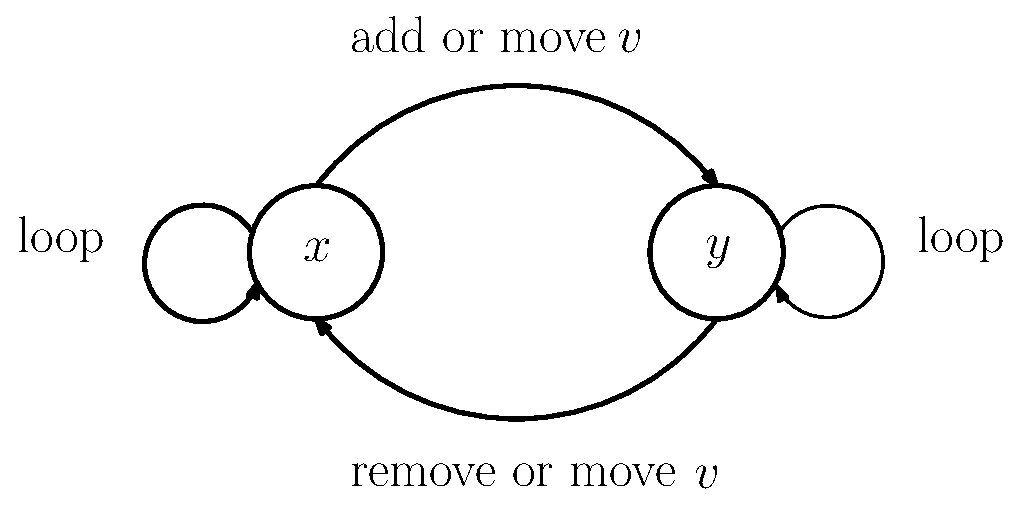
\includegraphics[scale=0.3]{assets/transition}
%     \caption{Transition relation between two states $x$ and $y$ in $\Omega$: either $y = x \cup \{v\}$ and $x = y - \{v\}$ or $v$ has been moved respectivly from $x$ to get $y/$ from $y$ to get $x$, where $v \in [0,k]^d$.}
%     \label{fig:fig2}
%   \end{center}
% \end{figure}

\begin{figure}
  \begin{center}
    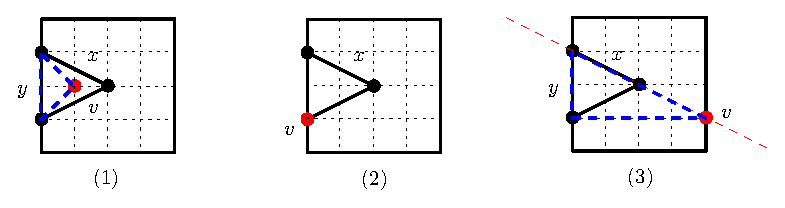
\includegraphics[scale=0.9]{assets/boucle}
    \caption{For $[0,4]^2$. Cases where we stay on $\p$: (1) $v$ is an interior point of $\p$, $P(\p,\p) = 1$. (2) $v$ is a vertex of $\p$, we stay on $\p$. (3) $v$ is drawn outside $Conv(\p)$ but $|Conv(\p\cup\{v\})| \neq |\p|+1$, $P(\p,\q) = 0$. }
    \label{fig:boucle}
  \end{center}
\end{figure}

\section{Properties of $(X_t)$}

The purpose of this paper is to build the random sampler of $(d,k)$-polytopes, in order to achieve our goal, we need to ensure that the stationnary distribution on $\Omega$ is the uniform. An important result on Markov chains shows that an irreducible, aperiodic and symetric Markov chain admits as stationnary distribution the uniform \cite{levin2009markov}.

This section aim to verify these properties on $(X_t)$, and give our first results on $(X_t)$. Only verifying the irreducibility has been slightly tricky, the other ones can be directly proved. In order to do so, the notion of symetric difference on our states will be introduced. Thereby, given $x$ and $y \in \Omega$, we recall that their \textit{symetric difference}, $x \bigtriangleup y$, is defined as:

\begin{equation}
  x \bigtriangleup y = x \cup y \setminus x \cap y
\end{equation}

% Here the symetric difference applied on two polytopes can be viewed in the same way as in the set theory, $x \bigtriangleup y = x \cup y \setminus x \cap y$, nevertheless some remarks worth mentioning:
%
% \begin{itemize}
%   \item $x \cup y$ is not always a convex hull.
%   \item $x \bigtriangleup y = x \setminus y \cup y \setminus x$
%   \item $|x \cup y| = |x| + |y|$ if $x \cap y = \emptyset$.
%   \item $x \bigtriangleup y$ is maximal when $x$ and $y$ do not have any common vertices.
% \end{itemize}

  Recall that the irreducibility mean that all the states of $\Omega$ can be reached from any other state, thus the irreducibility guarantees that the graph with vertex set $\Omega$ is connected. In fact move from $x$ to $y$ in our chain consists in finding finite number of transitions between $x$ and $y$ by one. Observe that the simplest way to move from $x$ to $y$ consists in adding directly to $x$ the vertices of $y$ then remove $x$ vertices. This means that at each step one reduces the symetric difference between $x$ and $y$. Hence, one can verify that the cardinality of $x \bigtriangleup y$ is a lower bound for the distance, noted $\delta(x,y)$, between $x$ and $y$. One has:

\begin{equation}
  \delta(x,y) \geq{|x \bigtriangleup y|}
\end{equation}

However, we might face cases which not allow this fast transition, thus we have to find out other transition state instead of those \textit{trivial} cases. Let us take into account the difficult cases and introduce lemmas to build our proof to the irreducibility. Not being able to add a point $w \in y \setminus x$ to $x$ means that for all $w \in y \setminus x$ the following cases occur: $w$ is an interior point to $x$, $w$ belongs to the affine hull of the edge of $x$, $v$ belongs to the cone described by one vertex of $x$ and the two edges which contains this vertex. To overcome this problem, we claim that we can always find a point $v$ in $[0,k]^d$ we can add to $x$, have a new state from wich we are building the path to $y$, then ensure the irreducibility.

\subsection{Existence of $v$}

% Lionel
Consider a $d$-dimensional lattice $(d,k)$-polytope $\S$ and assume that $\S$ is a simplex. Let $\mathcal{V}$ be the set of vertices of $\S$. For any $u\in\mathcal{V}$, denote by $H_u$ the affine hull of the facet of $\S$ opposite $u$, and by $H_u^-$ the closed half-space of $\mathbb{R}^d$ limited by $H_u$ that does not contain $u$.
For any $v\in\mathcal{V}$, the set

\begin{equation}
  C_v=\bigcap_{u\in\mathcal{V}\mathord{\setminus}\{v\}}H_u^-
\end{equation}

is a $d$-dimensional cone pointed at $v$. This cone is exactly the set of the points $x\in\mathbb{R}^d$ such that the convex hull of $\S\cup\{x\}$ does not admit $v$ as a vertex. By this remark, we have the following lemma.

\begin{lemma}\label{Lem.A}
Let $x$ be a lattice point in $[0,k]^d$. The convex hull of $\S\cup\{x\}$ admits, as vertices, $x$ and all the vertices of $\S$ if and only if $x$ does not belong to $\S$ and, for all $v\in\mathcal{V}$, $x$ does not belong to $C_v$.
\end{lemma}

Call $\gamma=\min\{x_1:x\in{S}\}$. Consider the following hyperplane of $\mathbb{R}^d$:
$$
X=\{x\in\mathbb{R}^d:x_1=\gamma\}
$$

Denote by $X^-$ the open half-space of $\mathbb{R}^d$ bounded by $X$ and that does not contain $\S$. By construction, the intersection $\S\cap{X}$ is a non-empty, proper face of $\S$. This face will be denoted by $F$ in the following. Since $\S$ is a simplex, it admits another, non-empty face $F^\star$ whose vertices are exactly the vertices of $\S$ that do not belong to $F$.

By construction,
$$
\mathrm{dim}(F)+\mathrm{dim}(F^\star)=d-1\mbox{.}
$$

In particular, there exists a vector $c$ that is orthogonal to both $F$ and $F^\star$. Consider the hyperplane $Y$ of $\mathbb{R}^d$ that admits $c$ as a normal vector and such that $F^\star\subset{Y}$. The intersection $\S\cap{Y}$ is precisely $F^\star$. Denote by $Y^-$ the closed half-space of $\mathbb{R}^d$ bounded by $Y$ that does not contain $F$. It will be assumed that $c$ has norm $1$ and that it points towards $Y^-$. Let
\begin{equation}\label{eq.A}
\delta=\min\{c\mathord{\cdot}x:x\in{X\cap[0,k]^d}\}\mbox{.}
\end{equation}

Further denote $G=\{x\in{X\cap[0,k]^d}:c\mathord{\cdot}x=\delta\}$. In the statement of the following lemma, $\mathrm{aff}(F)$ denotes the affine hull of $F$.

\begin{lemma}\label{Lem.B}
  If $v$ is a vertex of $\S$, then
  $$
  C_v\subset\mathrm{aff}(F)\cup{X^-}\cup{Y^-}\mbox{.}
  $$
\end{lemma}

\begin{proof}
  First observe that, if $s$ is a face of $\S$ and $H$ is a hyperplane of $\mathbb{R}^d$ that intersects $\S$ exactly along $s$, then
  $$
  \bigcap_{u\in\mathcal{V}\mathord{\setminus}s}H_u^-\subset{H^-}\mbox{,}
  $$
  where $H^-$ is the closed half space of $\mathbb{R}^d$ bounded by $H$ and disjoint from the interior of $\S$. Further observe that the intersection of $H$ with
  $$
  \bigcap_{u\in\mathcal{V}\mathord{\setminus}s}H_u^-
  $$
  is precisely the affine hull of $\S$. As a direct consequence, taking in turn $s=F^\star$ and $s=F$, one obtains that, if $v$ is a vertex of $F$, then $C_v\subset\mathrm{aff}(F)\cup{X^-}$ and if $v$ is a vertex of $F^\star$, then $C_v\subset{Y^-}$. The result therefore holds because any vertex of $\S$ is either a vertex of $F$ or a vertex of $F^\star$.
\end{proof}

As an immediate consequence of this and Lemma \ref{Lem.A}, for any lattice point $x\in[0,k]^d$ that does not belong to $X^-$, to $Y^-$, or to the affine hull of $F$, the convex hull of $\S\cup\{x\}$ admits, as vertices, $x$ and all the vertices of $\S$.

Recall that $c$ is orthogonal to $F$ and $F^\star$. As a consequence, the map $x\mapsto{c\mathord{\cdot}x}$ is constant within $F$ and within $F^\star$. Call $\varepsilon$ the value of $c\mathord{\cdot}x$ when $x\in{F}$ and $\varepsilon^\star$ the value of $c\mathord{\cdot}x$ when $x\in{F^\star}$. Since $F$ and $Y^-$ are disjoint, $\varepsilon<\varepsilon^\star$. Moreover, by (\ref{eq.A}), $\delta\leq\varepsilon$. Observe that if the latter inequality is strict, then $G$ is disjoint from both $\mathrm{aff}(F)$ and $Y^-$. By definition, it is also disjoint from $X^-$ and the following lemma is then obtained as a consequence of Lemmas \ref{Lem.A} and \ref{Lem.B}.
\begin{lemma}\label{Lem.BC}
If $\delta<\varepsilon$, then for any lattice point $x\in{G}$, the convex hull of $\S\cup\{x\}$ admits, as vertices, $x$ and all the vertices of $\S$.
\end{lemma}

If, on the contrary, $\delta$ and $\varepsilon$ coincide, then $F\subset{G}$. This situation is familiar: we are looking at a lattice simplex $F$ contained in a (possibly degenerate) lattice cube $G$. If the dimension of $G$ is greater than the dimension of $F$, then the following lemma provides the desired result.

\begin{lemma}\label{Lem.C}
If $k$ and $d$ are positive and if $P$ is a lattice $(d,k)$-polytope of dimension less than $d$ then there exists a lattice point $x$ that belongs to $[0,k]^d$ but that does not belong to the affine hull of $P$.
\end{lemma}
\begin{proof}
If $P$ is a lattice $(d,k)$-polytope of dimension less than $d$, then the intersection $I$ of its affine hull with $[0,k]^d$ cannot contain more than $(k+1)^{d-1}$ lattice points. Indeed, one can always project $I$ orthogonally on a facet of $[0,k]^d$ in such a way that the dimension of the projection is not less than that of $I$. Such a projection induces an injection from the lattice points in $I$ into the lattice points in the facet on which the projection is made.

Now observe that $[0,k]^d$ contains $(k+1)^d$ lattice points. Since $k$ is positive, $(k+1)^{d-1}<(k+1)^d$ and the lemma is proven.
\end{proof}

Hence, it remains to solve the case when $F$ is a subset of $G$ and both have the same dimension. If this dimension is at least $2$, then the strategy is to argue by induction on $d$. The base case of the induction is given by the following lemma.

\begin{lemma}\label{Lem.D}
If $d=2$ then there exists a lattice point $x\in[0,k]^2$ such that the convex hull of $\S\cup\{x\}$ admits, as vertices, $x$ and all the vertices of $\S$.
\end{lemma}
\begin{proof}
Probably just a careful, hopefully short disjunction. Rado, Julien?
\end{proof}

The case when $F$ is a subset of $G$ and their common dimension is either $0$ or $1$ has to be treated separately.

\begin{lemma}\label{Lem.E}
Assume that $d$ is greater than $2$. If $G$ has dimension at most $1$ and admits $F$ as a subset, then there exists at least one lattice point $x$ in $[0,k]^d$ that does not belong to $\mathrm{aff}(F)\cup{X^-}\cup{Y^-}$.
\end{lemma}
\begin{proof}
Assume that the dimension of $G$ is $0$ or $1$ and that $F$ is a subset of $G$. Because of the latter assumption, $\delta=\varepsilon$. Further assume that every lattice point in $X\cap[0,k]^d$ belongs to either $\mathrm{aff}(F)$ or $Y^-$. Since $Y^-$ is the set of points $x\in\mathbb{R}^d$ such that $c\mathord{\cdot}x\geq\varepsilon^\star$, this assumption yields that any lattice point $x$ in $X\cap[0,k]^d$
 such that $c\mathord{\cdot}x<\varepsilon^\star$ satisfies $c\mathord{\cdot}x=\delta$.

In particular, the only lattice points in $X\cap[0,k]^d$ that may belong to $Y$ have distance exactly $1$ to some lattice point in $G$.

Now consider the set $N$ of the points $x$ in $[0,k]^d$ whose orthogonal projection on $X$ belongs to $G$ and such that $x_i=\gamma+1$. By construction, $\gamma<k$ and therefore, $N$ is non-empty. More precisely, $N$ is made up of a single point if $G$ has dimension $0$, and $N$ is a line segment parallel to $G$ if $G$ has dimension $1$. In particular, the map $x\mapsto{c\mathord{\cdot}x}$ is constant within $N$. Call this constant $\eta$. If $\eta\geq\varepsilon^\star$
, then the only lattice points $x$ in $[0,k]^d$ such that $x_i\geq\gamma$ that may belong to $Y$ are the ones whose distance to some lattice point in $G$ is exactly $1$. Among these candidates, the only ones that can also be vertices of $\S$ are the lattice point in $N$. Indeed, all the other candidates belong to $X$. This is impossible because $\S$ would then be contained in the convex hull of $G\cup{N}$ whose dimension is either $1$ or $2$ depending on the dimension of $G$, whereas the dimension of $\S$ is at least $3$.

It follows from this contradiction that $\eta<\varepsilon^\star$. In other words, $N$ is disjoint from $Y^-$. By construction, $N$ is also disjoint from $X^-$ and from the affine hull of $F$. As $N$ contains lattice points, this proves the lemma.
\end{proof}

Here now comes the following proposition we want to claim.

\begin{proposition}\label{prop.A}
There exists a lattice point $x$ in the cube $[0,k]^d$ such that the convex hull of $\S\cup\{x\}$ admits, as vertices, $x$ and all the vertices of $\S$.
\end{proposition}

\begin{proof}
We need to write the induction carefully. Rado, Julien?
\end{proof}

\subsection{Irreducibility of $(X_t)$}

% A faire en lemme ou pas???

\begin{lemma}\label{lem:elim-mauvais-cas}
  For any simplex $x \in \Omega$, for any $y \in \Omega$. If we cannot reduce $x \bigtriangleup y$ by adding a vertex in $y \setminus x$ the there exists a simplex $z \in \Omega$, a transition state between $x$ and $y$, which verifies:
  \begin{itemize}
    \item $|x \bigtriangleup y| = |z \bigtriangleup y|$
    \item $\delta(x,z)\leq{2}$
  \end{itemize}
  such that we can always add a vertex in $y \setminus z$, from $z$ to $y$.
\end{lemma}

\begin{proof}
Let be $x$ a simplex $y$ be in $\Omega$. Let be $v \in [0,k]^d$. The idea of the proof lies on the fact that, $z$ will be found by adding a point $v \in \Omega$ and which is not an element of $x \bigtriangleup y$, then remove a point of $x \setminus y$. In this way we found the simplex $z$ at most in 2 steps.
\end{proof}

\begin{lemma}\label{lem:irreducibility}
  For all $x$ and $y \in \Omega$, there exists $z \in \Omega$ which satisfies $|x \bigtriangleup y| > |z \bigtriangleup y|$ such that $\delta(x,z)\leq{3}$.
\end{lemma}

\begin{proof}
  Let $x$ and $y$ be states of $\Omega$, such that $P(x,y)=0$. Let $z$ be a transition state between $x$ and $y$, and such that $z$ is closer to $y$ than $y$. We have several distinct cases:

  \begin{enumerate}
    \item $x$ is not a simplex.
    \begin{enumerate}
      \item $x \subset y$: add $v \in y \setminus x$ and $z = x \cup \{v\}$, then $\delta(x,z) = 1$
      \item $x \not\subset y$: remove $v \in x \setminus y$ and $z = x - \{v\}$, then $\delta(x,z) = 1$
    \end{enumerate}
    \item $x$ is a simplex.
    \begin{enumerate}
      \item If we can add $v \in y \setminus x$ then add it, thus $z = x \cup \{v\}$ and $\delta(x,z) = 1$
      \item Else:
      \begin{enumerate}
        \item Add a point $u$ which is not in $x \bigtriangleup y$
        \item Remove a point from  $x \setminus y$
        \item Add  a point from $y \setminus x$

        In this last case, one finds $z$ such that $\delta(x,z) = 3$
      \end{enumerate}
    \end{enumerate}
  \end{enumerate}

  Since we had proved we can always add a point which is not contained in $x \bigtriangleup y$ by lemma \ref{lem:elim-mauvais-cas}. It means that wherever in which case we are, one can always find a $z$ which reduces the symetric difference from $z$ to $y$ by one, such that $\delta(x,z) \leq{3}$.

\end{proof}

\begin{corollary}\label{coro:diameter}
  For all $x$ and $y \in \Omega$ one has:
  \begin{equation}
    \delta(x,y) \leq |x| + |y| + 4(d+1)
  \end{equation}
\end{corollary}

\begin{proof}
  This is an immediate consequence of the lemma \ref{lem:irreducibility}. Let $x$ and $y$ be in $\Omega$. Let us now consider two simplices $x^\star$ and $y^\star$ such that $\delta(x,x^\star) = |x| - (d+1)$, and $\delta(y,y^\star) = |y| - (d+1)$. Thus
  $$
    \delta(x,y) \leq{\delta(x,x^\star) + \delta(x^\star,y^\star) + \delta(y,y^\star)}
  $$
  Since $x^\star$ is a simplex, the walk needs at most $3(|x^\star| + |y^\star|) = 3 \times 2(d+1)$ steps to reach $y^\star$ from $x^\star$. Hence
  $$
    \delta(x,y) \leq{|x| - (d+1) + |y| - (d+1) + 6(d+1)} = |x| + |y| + 4(d+1)
  $$
\end{proof}

Observe that corollary \ref{coro:diameter} gives an idea on the upper bound of the diameter of $(X_t)$. We have now settled all we need to prove our main results on the properties of $(X_t)$.

\begin{theorem}\label{thm:diameter}
  Define the diameter $\mathcal{D}$ of a graph with vertex set $\Omega$ to be the maximum distance between two vertices. For $(X_t)$, as defined above, and given $k$ and $d$, one has:
  \begin{equation}
    \mathcal{D}_{X_t} \leq{2ck^{3/4} + 4(d+1)} \quad \mbox{where} \ c>0
  \end{equation}
\end{theorem}

\begin{proof}
  To be done.
\end{proof}

\begin{theorem}\label{thm:main}
  The Markov chain $(X_t)$ is irreductible, aperiodic and has the uniform as stationnary distribution.
\end{theorem}

\begin{proof}
  Three propreties have to be verified, thus this proof will be given in three steps. Let $x$ and $y$ be in $\Omega$.

  \begin{enumerate}[i]
    \item \textit{Irreducibility}
    Irreducibility is a direct consequence of the corollary \ref{coro:diameter}. Let us remind that to prove the irreducibility, one needs to find a $r_0$ such that, for all $x$ and $y \in \Omega$, when $r \geq{r_0}$ then $P^r(x,y)>0$. Thus let us take $r_0 = |x| + |y| + 4(d+1)$.

     \item \textit{Symetry}
     Our transition rules consists in either add or remove a single vertex for two distinct states. Observe that if there is no one step transition from $x$ to $y$ means $P(x,y)=0$. By the trasition rules, necessarily, if $P(x,y)=0$ then $P(y,x)=0$.
     Next, let us prove that if $P(x,y)>0$ and $P(y,x)>0$ then we also have $P(x,y) = P(y,x)$. $P(x,y)>0$ means that we have a one step transition from $x$ to $y$. Only two cases may occur. For $v \in [0,k^d]$ either $y = x - \{v\}$, or $y = x \cup \{v\}$. Considering the first case, the probability to draw $v$ and add it to $x$ is $P(x,y) = \frac{1}{(k+1)^d}$. Similarily, to move from $y$ to $x$, we draw the same $v$ and remove it from $y$ to get $x$ with probability $P(y,x) = \frac{1}{(k+1)^d} = P(x,y)$. We prove the remaining case in an analog reasoning.

     \item \textit{Aperiodicity}
     To prove that $(X_t)$ is aperiodic, one needs to show that each state in $\Omega$ has as period $1$. Since $(X_t)$ is irreductible, property \ref{prop:irr-ap} tells us that all the states of $\Omega$ has the same period. Thus, for all $x, y \in \Omega$, $\mathrm{gcd}(\mathcal{T}(x)) = \mathrm{gcd}(\mathcal{T}(y))$. One needs to find a state $x$ such that t$\mathrm{gcd}(\mathcal{T}(x)) = 1$. Let us take $x$ has a simplex and a point $v \in [0,k]^d$ then consider the cases where we have a loop on $x$:
     either $v$ is an interior point to $x$, or $v$ is drawn outside of $x$ but $|Conv(x \cup \{v\})| \neq |x| + 1$. One has: $P(x,x) = \mathbf{P}\{v \  \mbox{interior point to} \ x\} + \mathbf{P}\{v \in x\} + \mathbf{P}\{|x \cup \{v\}| \neq |x| + 1\}$.
     Note that $\mathbf{P}\{v \in x\} = \frac{1}{(k+1)^d}$, but since $|x| = d+1$, we have a loop on $x$ with probability $P(x,x) \geq{\frac{1}{(k+1)^d}} > 0$. In another words, with positive probability the walk can get back to $x$ from $x$ in one step. Hence, $\mathcal{T}(x) = \{1, \dots\}$. We conclude that $\mathrm{gcd}(\mathcal{T}(x)) = 1$.

   \end{enumerate}
\end{proof}

\section{Random sampler}

Consider $(X_t)$ as defined previously. Sampling random $(d, k)$-polytopes consists in a random walk on $\Omega$ with our transition rules until one reaches the stationnary distribution. The amount of time needed to reach such a distribution, that is sample a uniformally random $(d, k)$-polytope, is the mixing time on $(X_t)$.

Sampling a random $(d, k)$-polytope with this model is given the following algorithm.

\vspace{0.5cm}

\begin{algorithm}[H]\label{Algo.RS}
  \LinesNumbered
  \DontPrintSemicolon
  \KwIn{the dimension $d$, the size $k$ of the hypercube}
  \KwOut{a random lattice $(d,k)$-polytope}
  \BlankLine

  sample a random lattice $(d,k)$-simplex $P$ with vertex set $\mathcal{V}$\;
  \While{we are not close enough to the stationary distribution}{
  generate a random lattice point $x$ in $[0,k]^d$\;
  \If{$x \in \mathcal{V}$ and $\mathrm{conv}(\mathcal{V}\mathord{\setminus}\{x\})$ is $d$-dimensional}{
    $P \leftarrow \mathrm{conv}(\mathcal{V}\mathord{\setminus}\{x\})$\;
   }
  %\Else{$|\mathrm{conv}(\mathcal{V} \cup \{x\})|$ == $|\mathcal{V}| + 1$}{
  \Else{
    compute the convex hull $Q$ of $\mathcal{V}\cup\{x\}$\;
    \If{the vertex set of $Q$ is $\mathcal{V}\cup\{x\}$}{
      $P \leftarrow \mathrm{conv}(\mathcal{V} \cup \{ x\})$\;
    }
  }
 }
 \Return{$P$}
 \caption{Random sampling of a lattice $(d, k)$-polytope}
\end{algorithm}


\begin{theorem}\label{thm:random-sampler}
  The random sampler $\Gamma(d,k)$ described by algorithm \ref{algo1} is a uniform random sampler of $(d,k)$-polytopes over $\Omega$.
\end{theorem}

\section{Results on mixing time}



\clearpage
\bibliographystyle{plain}
\bibliography{biblio.bib}

\end{document}
